\documentclass[]{llncs}

%% The amssymb package provides various useful mathematical symbols
\usepackage{amssymb}
%% The amsthm package provides extended theorem environments
%\usepackage{amsthm}
\usepackage{amsmath}

%% for url reference
\usepackage{hyperref}
\usepackage{graphicx}

\usepackage{float}
\def\infinity{\rotatebox{90}{8}}

\newcommand{\texp}{|\Delta|}
\newcommand{\block}{\mathcal{B}}
\newcommand{\reward}{\mathcal{W}}
\newcommand{\cost}{\mathcal{C}}

\newcommand{\attackname}{coin-hopping attack}
\newcommand{\AttackName}{Coin-hopping Attack}


\begin{document}


\title{[Short Paper:] Revisiting Difficulty Control for Blockchain Systems}


\author{Dmitry Meshkov \and Alexander Chepurnoy}
\institute{IOHK Research}

%\ead{dmitry.meshkov@iohk.io}

\maketitle

\begin{abstract}

The Bitcoin whitepaper~\cite{Nakamoto2008} states that the security of the system is guaranteed as long as honest miners control more than half of the current total computational power. The whitepaper assumes static difficulty case when it is equally hard to solve a cryptographic proof-of-work puzzle dependless on system behavior. However, a real Bitcoin network is using an adaptive difficulty adjustment mechanism.  

In this paper we introduce and analyze a new kind of attack on mining difficulty retargeting. A malicious miner is increasing his mining profits from the attack. An average time interval between blocks is increasing as a side-effect of the attack.

We propose an alternative difficulty adjustment algorithm in order to reduce an incentive to attack and also to improve stability of inter-block delays. We show that the novel approach performs better than original algorithm of Bitcoin.
	
\end{abstract}


\section{Introduction}
\label{sec:intro}

Blockchain systems have attracted significant amount of interest after the Bitcoin whitepaper~\cite{Nakamoto2008} was published in 2008.
Bitcoin security relies on a distributed protocol which maintains a distributed ledger. In the protocol miners are trying to find a partial hash collision in order to generate a valid block by iterating over nonce field values. That is, for a block $\block$~(with a random nonce included) to be valid, condition $hash(\block) < T$ should hold, where {\em target} parameter $T$ specifies expected hardness of a valid block generation. This hardness can be also viewed via {\em difficulty} parameter $D = \frac{1}{T}$.

Alternative systems may rely on different than finding a partial hash collision types of computational puzzles~\cite{miller2014permacoin,biryukov2017equihash}. Nevertheless, all of them assume some algorithm that changes puzzle difficulty dynamically. The algorithm for difficulty readjustment is required in order to make an open blockchain system working stable in the face of participants joining and leaving the system, and also to stabilize mean latency between blocks. 

A difficulty readjustment algorithm in Bitcoin assumes that total computational power involved in mining process does not significantly change from epoch to epoch. In contrast, real networks show that significant variance in computational power could happen for long periods.
For example, we show in this paper that due to continuous growth of computational power in Bitcoin network a mean delay between blocks by 7\% less than expected value.
Noteworthy, exponential growth of computational power, often observed in practice, is the absolutely worst case~(regarding the mean block delay divergence) for the Bitcoin’s difficulty readjustment algorithm~\cite{kraft2015difficulty}.
 
In this paper we also consider a new type of miner behavior in regards with difficulty readjustment problematic for security guarantees of a blockchain system which we call a \attackname following the ``pool-hopping'' term raised in~\cite{rosenfeld2011analysis}. In this attack, an adversarial miner is switching from mining one coin to another in the beginning of an epoch, then he is switching back in the beginning of next epoch when difficulty becomes lower. We show how mining profit is increasing for Bitcoin's difficulty readjustment function, and how inter-block delay suffer from the \attackname.

As a solution for significant variance in computational power and also in order to reduce incentive to follow coin-hopping strategy, we propose an alternative difficulty readjustment procedure. The new algorithm is using integer arithmetic for all the steps only, which is important since nodes in peer-to-peer network are running on different platforms. We show that the proposed solution is better suited for exponential growth of total mining power and also reduces profit and negative side-effects of the coin-hopping attack.

\subsection{Related Work}

Here we observe known formal and informal studies of Bitcoin in regards with dynamic nature of difficulty parameter. Following the well known paper of Garay et al.~\cite{garay2015bitcoin} generalizing Bitcoin backbone protocol in static difficulty setting, a newer paper from the same authors~\cite{gkl16} is getting positive answer on whether basic security properties of the Bitcoin backbone protocol~(common prefix, chain quality and chain growth) hold in case of dynamic difficulty, in a cryptographic setting with an arbitrary adversary. Nevertheless, studying concrete attacks against the real protocol is still needed.      

Timejacking attack~\cite{timejacking2011} allows an attacker first shift network time at a victim node~(which is calculating network time by averaging timestamps got regularly from neighbors) and then force the victim node to reject a block with a specially crafted timestamp~(other nodes are accepting). The time wrapping attack~\cite{artforz2011} is exploiting the fact Bitcoin is using difference in timestamps between last and first block in an epoch, not last block in an epoch and last block in a previous epoch. By using specially crafted timestamps for the last block of each epoch, an attacker can produce more blocks for a time window with more work contributed to his chain. The difficulty raising attack, introduced in~\cite{bahack2013theoretical}, allows an attacker to discard $n$-depth block, for any $n$, and for any computational power of the attacker, with probability 1 if he is willing to wait enough time.

A paper~\cite{kraft2015difficulty} is introducing an alternative difficulty readjustment function designed to work better than Bitcoin's not just for almost constant mining power but also when the power is growing exponentially with time. We provide comparison with this function in the paper.  

\subsection{Structure of the Paper}

Several parts are organizing the paper. In Section~\ref{sec:bit} we provide detailed view of Bitcoin readjustment function. In Section~\ref{sec:attack} we introduce the coin-hopping attack. In Section~\ref{sec:improved} an improved difficulty readjustment function is proposed and analyzed. Section~\ref{sec:sim} provides results of simulations. 

\section{Bitcoin Mining}
\label{sec:bit}

The concept of Bitcoin mining was introduced in the Section 4 of the Bitcoin whitepaper~\cite{Nakamoto2008} and discussed then in the papers~\cite{kraft2015difficulty},\cite{gkl16}. In Bitcoin a miner generates a block by iterating over {\em nonce} value and calculating hash of a block with the nonce value included. For a block $\block$ to be valid, a value of a hash function for it must be less than the current {\em target} $T$, $hash(\block) < T$, where $hash$ is an ideal cryptographic hash function. Hardness to find a block could be expressed also via {\em difficulty} $D$ as $D = \frac{1}{T}$. If output of $hash$ function is $\mu$ bits long then the probability to generate a block by doing $q$ requests to the hash function is $\frac{T \cdot q}{2^\mu} = \frac{q}{D \cdot 2^\mu}$. We define miner \textit{hashrate} $R$ as $R = \frac{q_s}{2^\mu}$, where $q_s$ is number of queries done per time unit. The probability to generate a block within time unit then is $\frac{R}{D}$.


Every $M$ blocks ($M = 2016$ for Bitcoin) difficulty is recalculated as
\begin{equation}
D_{i+1}=D_i \cdot {M \cdot \texp \over S_m}
\end{equation}
where $\texp$ is expected time interval between blocks and $S_m$ is actual time spent to generate $M$ blocks.
For Bitcoin observed time interval $\approx${\em 9 minutes 20 seconds} is less than planned value $\texp = 10$ {\em minutes} due to continuous growth of network computational power.
Difficulty recalculation interval $M=2016$ has been chosen to recalculate difficulty every 2 weeks on average.
This time interval is big enough to see computational power of the network being usually increased over it: right after target recalculation mean delay is close to planned 10 minutes, whereas at the end of an epoch it is less than 9 minutes in average (see Figure~\ref{fig:image}).

\begin{figure}[H]
\center{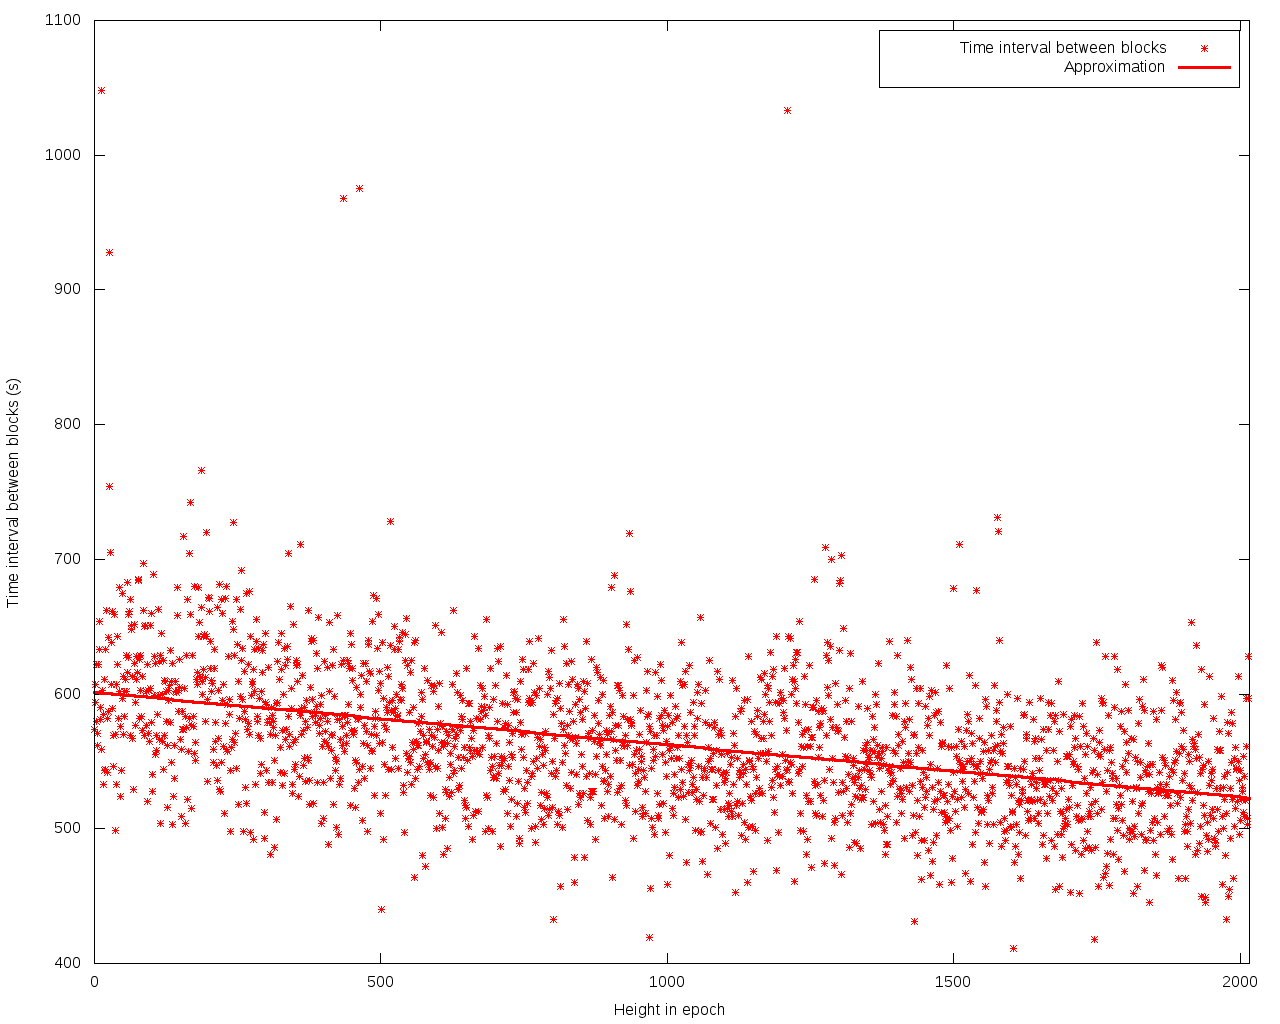
\includegraphics[scale=0.25]{interval.png}}
\caption{Average block time between difficulty recalculation}
\label{fig:image}
\end{figure}

\textbf{TODO the picture above is a mess}
\textbf{TODO transition to next section}

\section{\AttackName}
\label{sec:attack}

We consider the following attack involving an adversarial miner $\mathcal{A}$:

\begin{itemize}
\item There are $N > 1$ possible coins $\mathcal{A}$ can contribute to. Without a loss of generality, we assume that each of them is about the same profitability of the mining activity. 
\item $\mathcal{A}$ is mining one of the coins before a beginning of an epoch, say, epoch $A$. At the beginning of $A$ he switches to mine other coins. 
\item Without a contribution of $\mathcal{A}$ total mining power of the network for the epoch goes down. 
\item For an epoch $B$ next to the epoch $A$ difficulty readjusted to a lower value. So $\mathcal{A}$ starts mining again with a lower difficulty. 
\end{itemize}

We call this strategy a \textit{\attackname}.

To calculate adversarial profit from the attack we assume Bitcoin difficulty recalculation function and constant network hashrate. We denote hashrate of miners not participating in coin-hopping attack as $R_0$, and we denote adversarial hashrate as $R_a=R_0\cdot p, 0 < p < 1 $.
Before epoch $A$ the difficulty $D_0 = (R_0+R_a) \cdot \texp$, and the adversary mines $M \cdot R_a \over R_0 + R_a$ blocks per epoch (of $M$ blocks) in average by spending $M \cdot R_a \cdot \texp$ computational power for them.
During the epoch B the adversary mines with difficulty $D_1 = R_0 \cdot \texp$ calculated from honest miners hashrate $R_0$ only.
The adversary mines $M \cdot R_a \over 2(R_0+ R_a)$ blocks per epoch in average spending $M\cdot T\cdot R_a\cdot R_0\over 2 \cdot (R_0+R_a)$ computational power for them.
Consequently honest miner will spend $(R_0+R_a) \texp$ computational power per block, whereas attacker will just spend $R_0 \cdot \texp$ computational power per block.
The cost of computational resources invested into mining should be around the expected reward.
If $\reward$ is block reward and $\cost$ is hash calculation cost, the honest miner profit is
\begin{equation}
{({M \cdot R_a \over R_0 + R_a}) \cdot \reward - M \cdot R_a \cdot T \cdot \cost = M\cdot R_a\cdot ({\reward \over R_0+R_a}-T \cdot \cost)}
\end{equation}
per epoch.
At the same time adversarial profit is
\begin{equation}
{{M\cdot R_a \over 2\cdot (R_0+R_a)}\cdot (\reward - T\cdot R_0\cdot \cost)}
\end{equation}


Additional profit of the adversary is:
[TODO: ???]
\begin{equation}
{{\reward \over \cost} < T\cdot (R_0 + 2\cdot R_a)}.
\end{equation}



Remarkable, that under such an attack mean time between blocks will be
\begin{equation}
\label{eq:ati}
{T_a={T\over 2}({R_0+R_a\over R_0} + {R_0\over R_0+R_a})=T(1 + {p^2\over 2(1+p)})}
\end{equation}
which is bigger than the planned time $T$.

%Please notice that we regard \(p\) as the ratio between the hash-powers of the attacker and the honest network so it changes from 0 to 1.

\textbf{TODO transition to next section}



\section{Improved Difficulty Adjustment}
\label{sec:improved}

The difficulty adjustment algorithm employed by Bitcoin works as designed: if the hash rate of the network is constant, it yields the desired block rate. However it does not achieve the desired block rate in other situations and vulnerable to attack, described in \ref{sec:attack}.
In this section we are going to propose an alternative difficulty adjustment algorithm that works better than the Bitcoin's.

First, we state properties of an ideal difficulty update algorithm:
\begin{enumerate}
\item{It should be resistant to known types of attacks based on difficulty manipulation.}
\item{It should lead to desired block rate for random fluctuations in the hash rate.}
\item{It should be simple enough to use integer arithmetic for all computational steps.}
\end{enumerate}

Security is the most important feature of blockchain systems and should be regarded with the highest priority.
Incorrect block rate is not considered a big problem in the Bitcoin community but it may be important for more advanced applications of blockchain systems.
Implementation of the \textit{ideal} difficulty update algorithm in subclass of integer programming is desired for different platforms compatibility.
This rule is not required, because, as mentioned in \cite{kraft2015difficulty}, it is possible to include non-integer algorithm parameters as part of the block, but it provides another way of difficulty manipulating to an attacker.

In this section we are going to regard difficulty adjustment algorithm based on well-known linear least squares method\cite{lawson1974solving}. In the simpliest case of pair linear regression (\(y=kx+b)\) coefficients may be calculated as follows:

\begin{equation}
  \begin{cases}
    k= {{\overline{xy} - \overline{x}\overline{y}} \over {\overline{x^2} - \overline{x}^2}}  \\
    b= \overline{y}-k\overline{x}
  \end{cases}
\end{equation}

Note, that for accurate difficulty prediction we should use few last observed difficulties, rather than just one, as implemented in Bitcoin, but it's possible to use this algorithm right after second epoch.


We regard it as the good candidate for difficulty update algorithm, because:
\begin{enumerate}
\item{It should reduce profit of the attack, described in Section~\ref{sec:attack}. Calculations of the attacker profit are described in Section~\ref{sec:sim}}
\item{It leads to desired block rate for linear changes in the hash rate.
This means, that regarding block rate, linear algorithm is better, then Bitcoin's one, in all cases, except constant hash rate, when they lead to the same result. }
\item{It is simple enough to use integer arithmetic for all computational steps with high fidelity.}
\end{enumerate}

\section{Simulations}
\label{sec:sim}

We present simulation results that show how our method proposed in Section~\ref{sec:improved} improves over Bitcoin’s difficulty update algorithm.
We will regard \textit{difficulty} growth in this section, keeping in mind the fact, that it's closely related with network hash rate, which is usually considered in literature.

%All calculations have been performed with open-sourced programs, available at Scorex project GitHub page~\cite{scorex}.

\textbf{TODO Linear?}

\subsection{Exponential Difficulty}

First, we observe exponential difficulty growth occurred in practice in Bitcoin network. As we already mentioned, exponential difficulty growth is the absolutely worst case possible for Bitcoin’s difficulty retargeting algorithm.
For simplicity we regard a situation, when hash rate growth 10\% each epoch, more complicated research of exponential difficulty growth can be found in~\cite{kraft2015difficulty}.
Figure~\ref{fig:exp} presents difficulty as the function of epoch, which is 2016 blocks in Bitcoin.

\begin{figure}[h]
\center{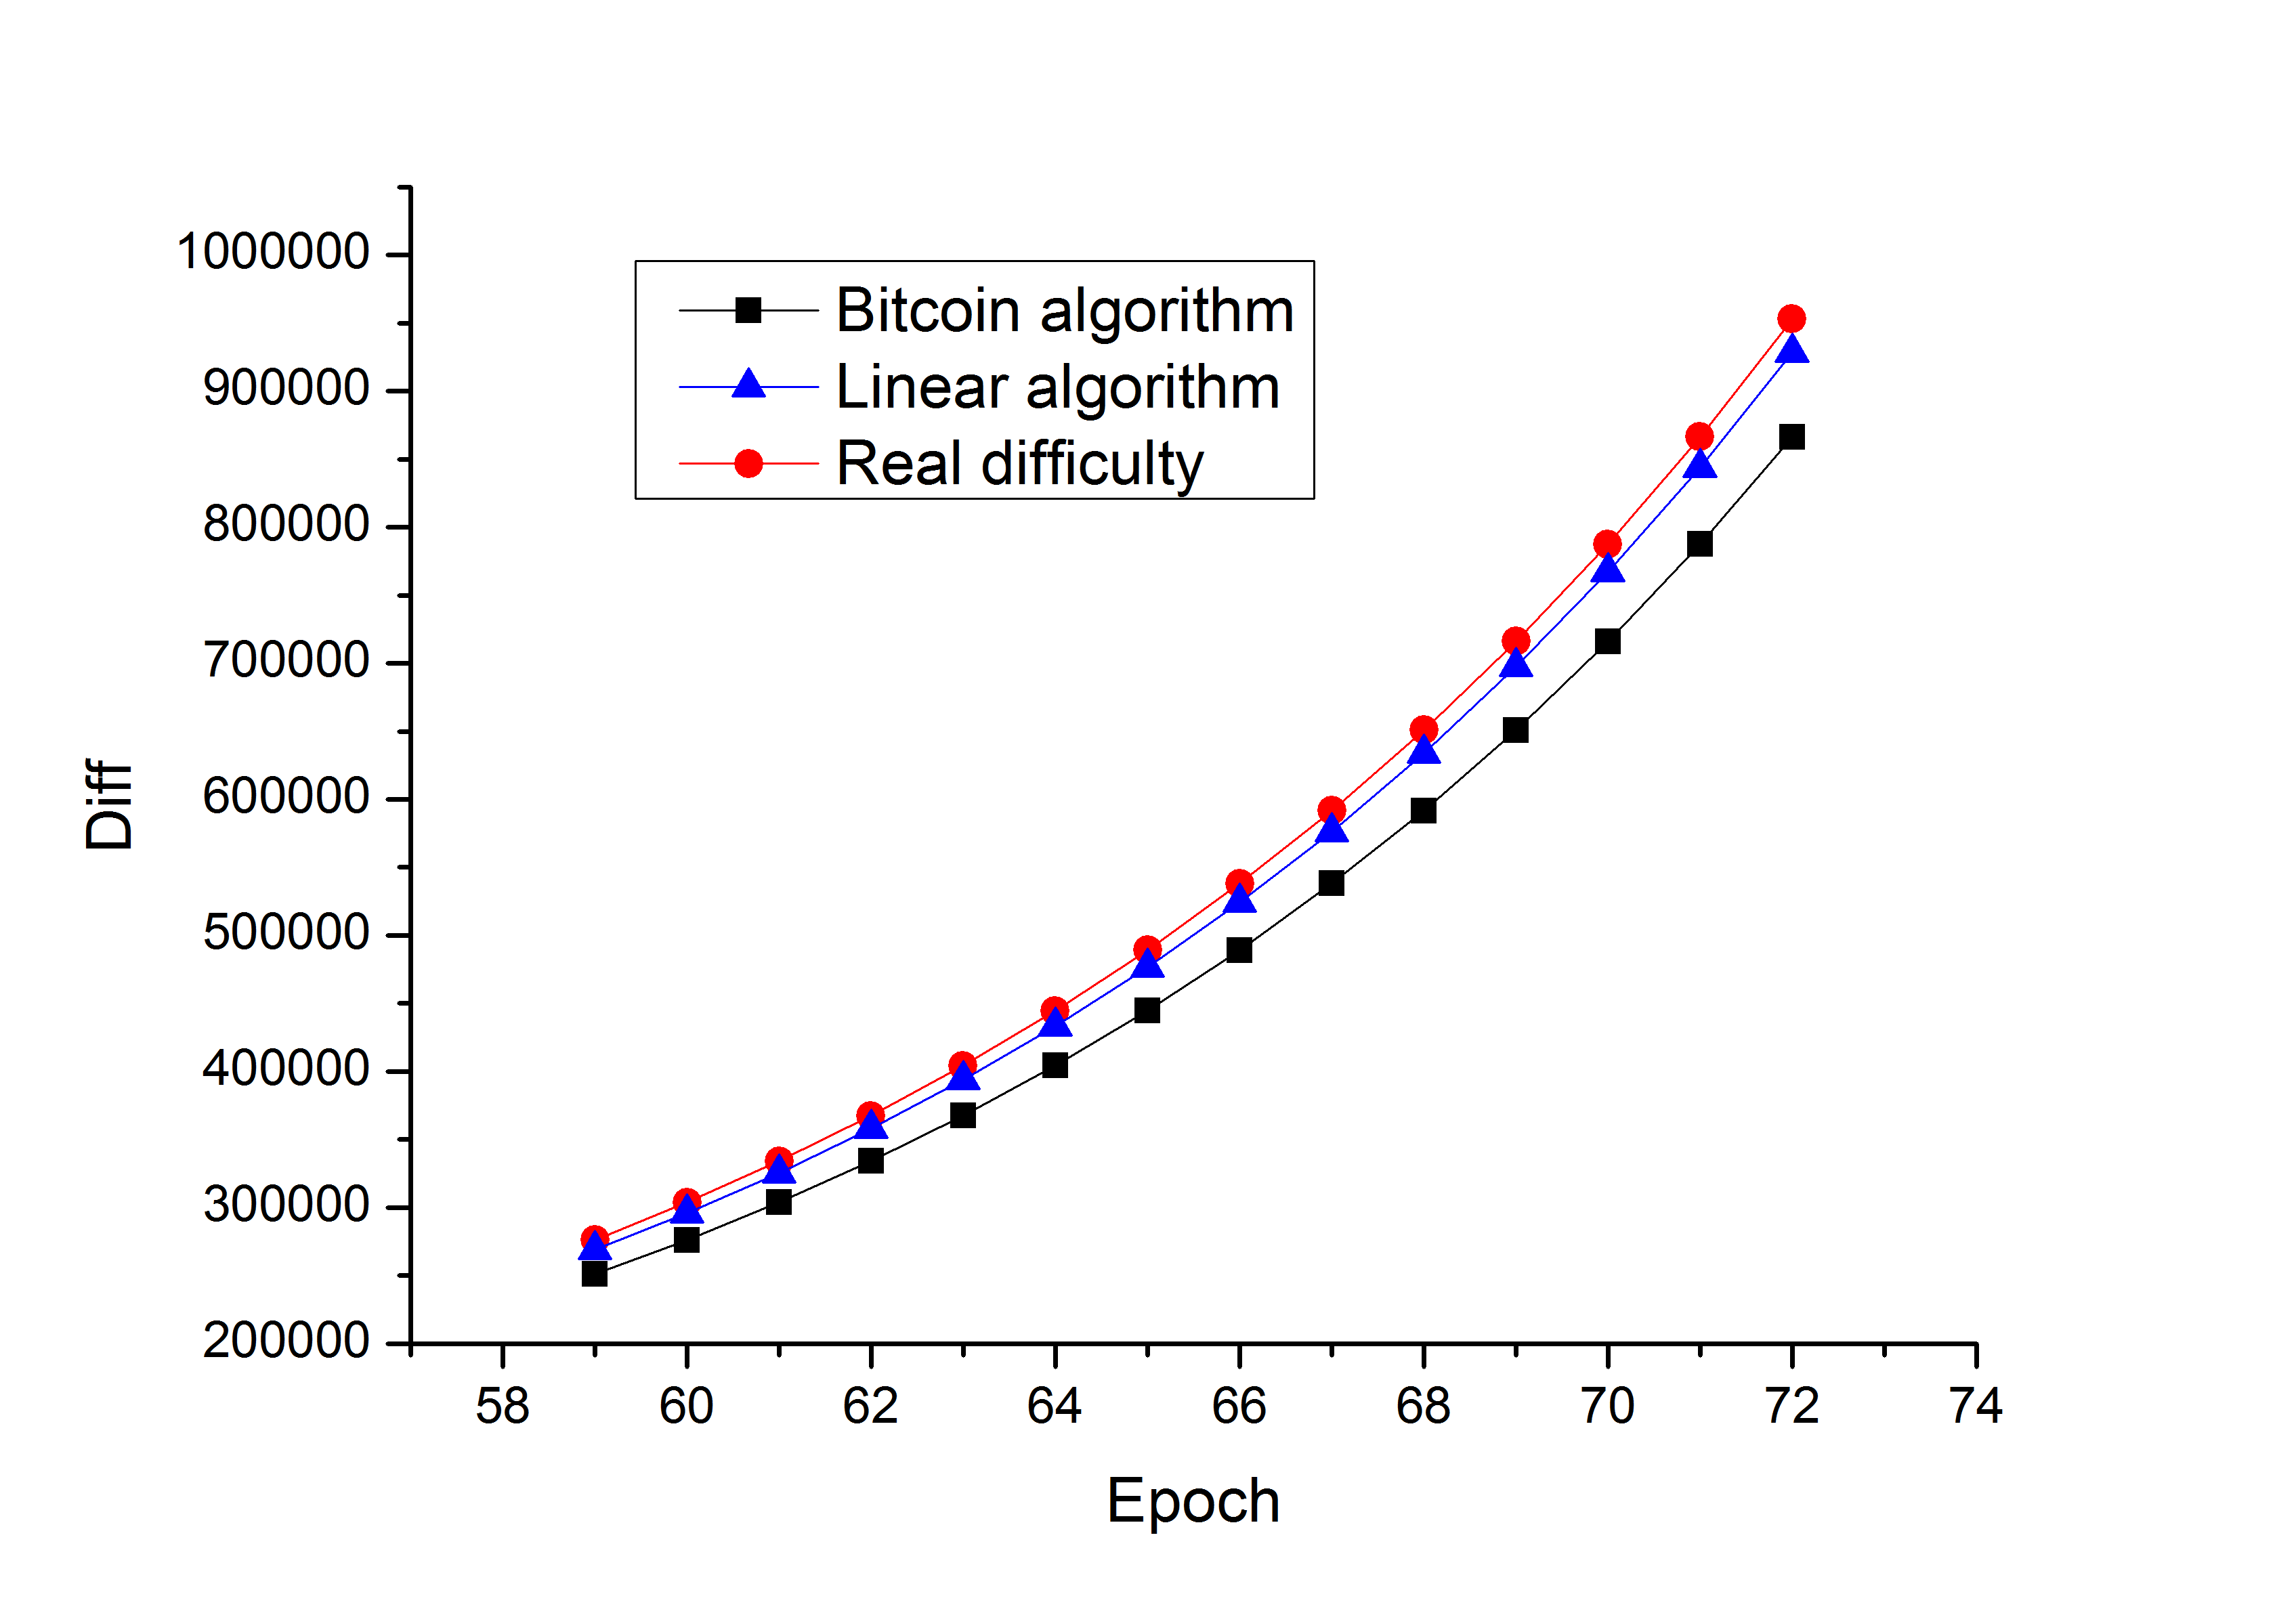
\includegraphics[scale=0.3]{exp.png}}
\caption{Real difficulty (red) and difficulties calculated from bitcoin (black) and linear (blue) algorithms in situation of exponential hash rate growth}
\label{fig:exp}
\end{figure}

Note that difficulty calculated from Bitcoin algorithm is always significantly lower than the real one.
This leads to \textit{9 min 5 sec} time interval between blocks, which is $\approx$10\% lower then desired \textit{10 min} interval.
Difficulty, calculated from Linear algorithm is also always lower, then the real one, while it's much closer to it.
Mean time interval between blocks is \textit{9 min 45 sec}, which is much closer to the desired one.

While difficulty update algorithm, proposed in~\cite{kraft2015difficulty} leads to much better results for exponential difficulty growth with a constant rate, we should note, that our algorithm is much simplier and may be implemented with integer arithmetic only.
Moreover, exponential difficulty growth is the simplification of the difficulty growth law, and it may be incorrect to expect it in some situations.

\subsection{\AttackName}

We consider a situation described in the Section~\ref{sec:attack}: an attacker with computational power \(R_a\) (for simplicity we suppose \(R_a=0.2 \cdot R_a \) in this section) turn on and turn off his mining to manipulate difficulty and minimize computational power, expended for block mining.
Figure \ref{fig:exp} represents difficulty as the function of epcoh for this situation.

\begin{figure}[h]
\center{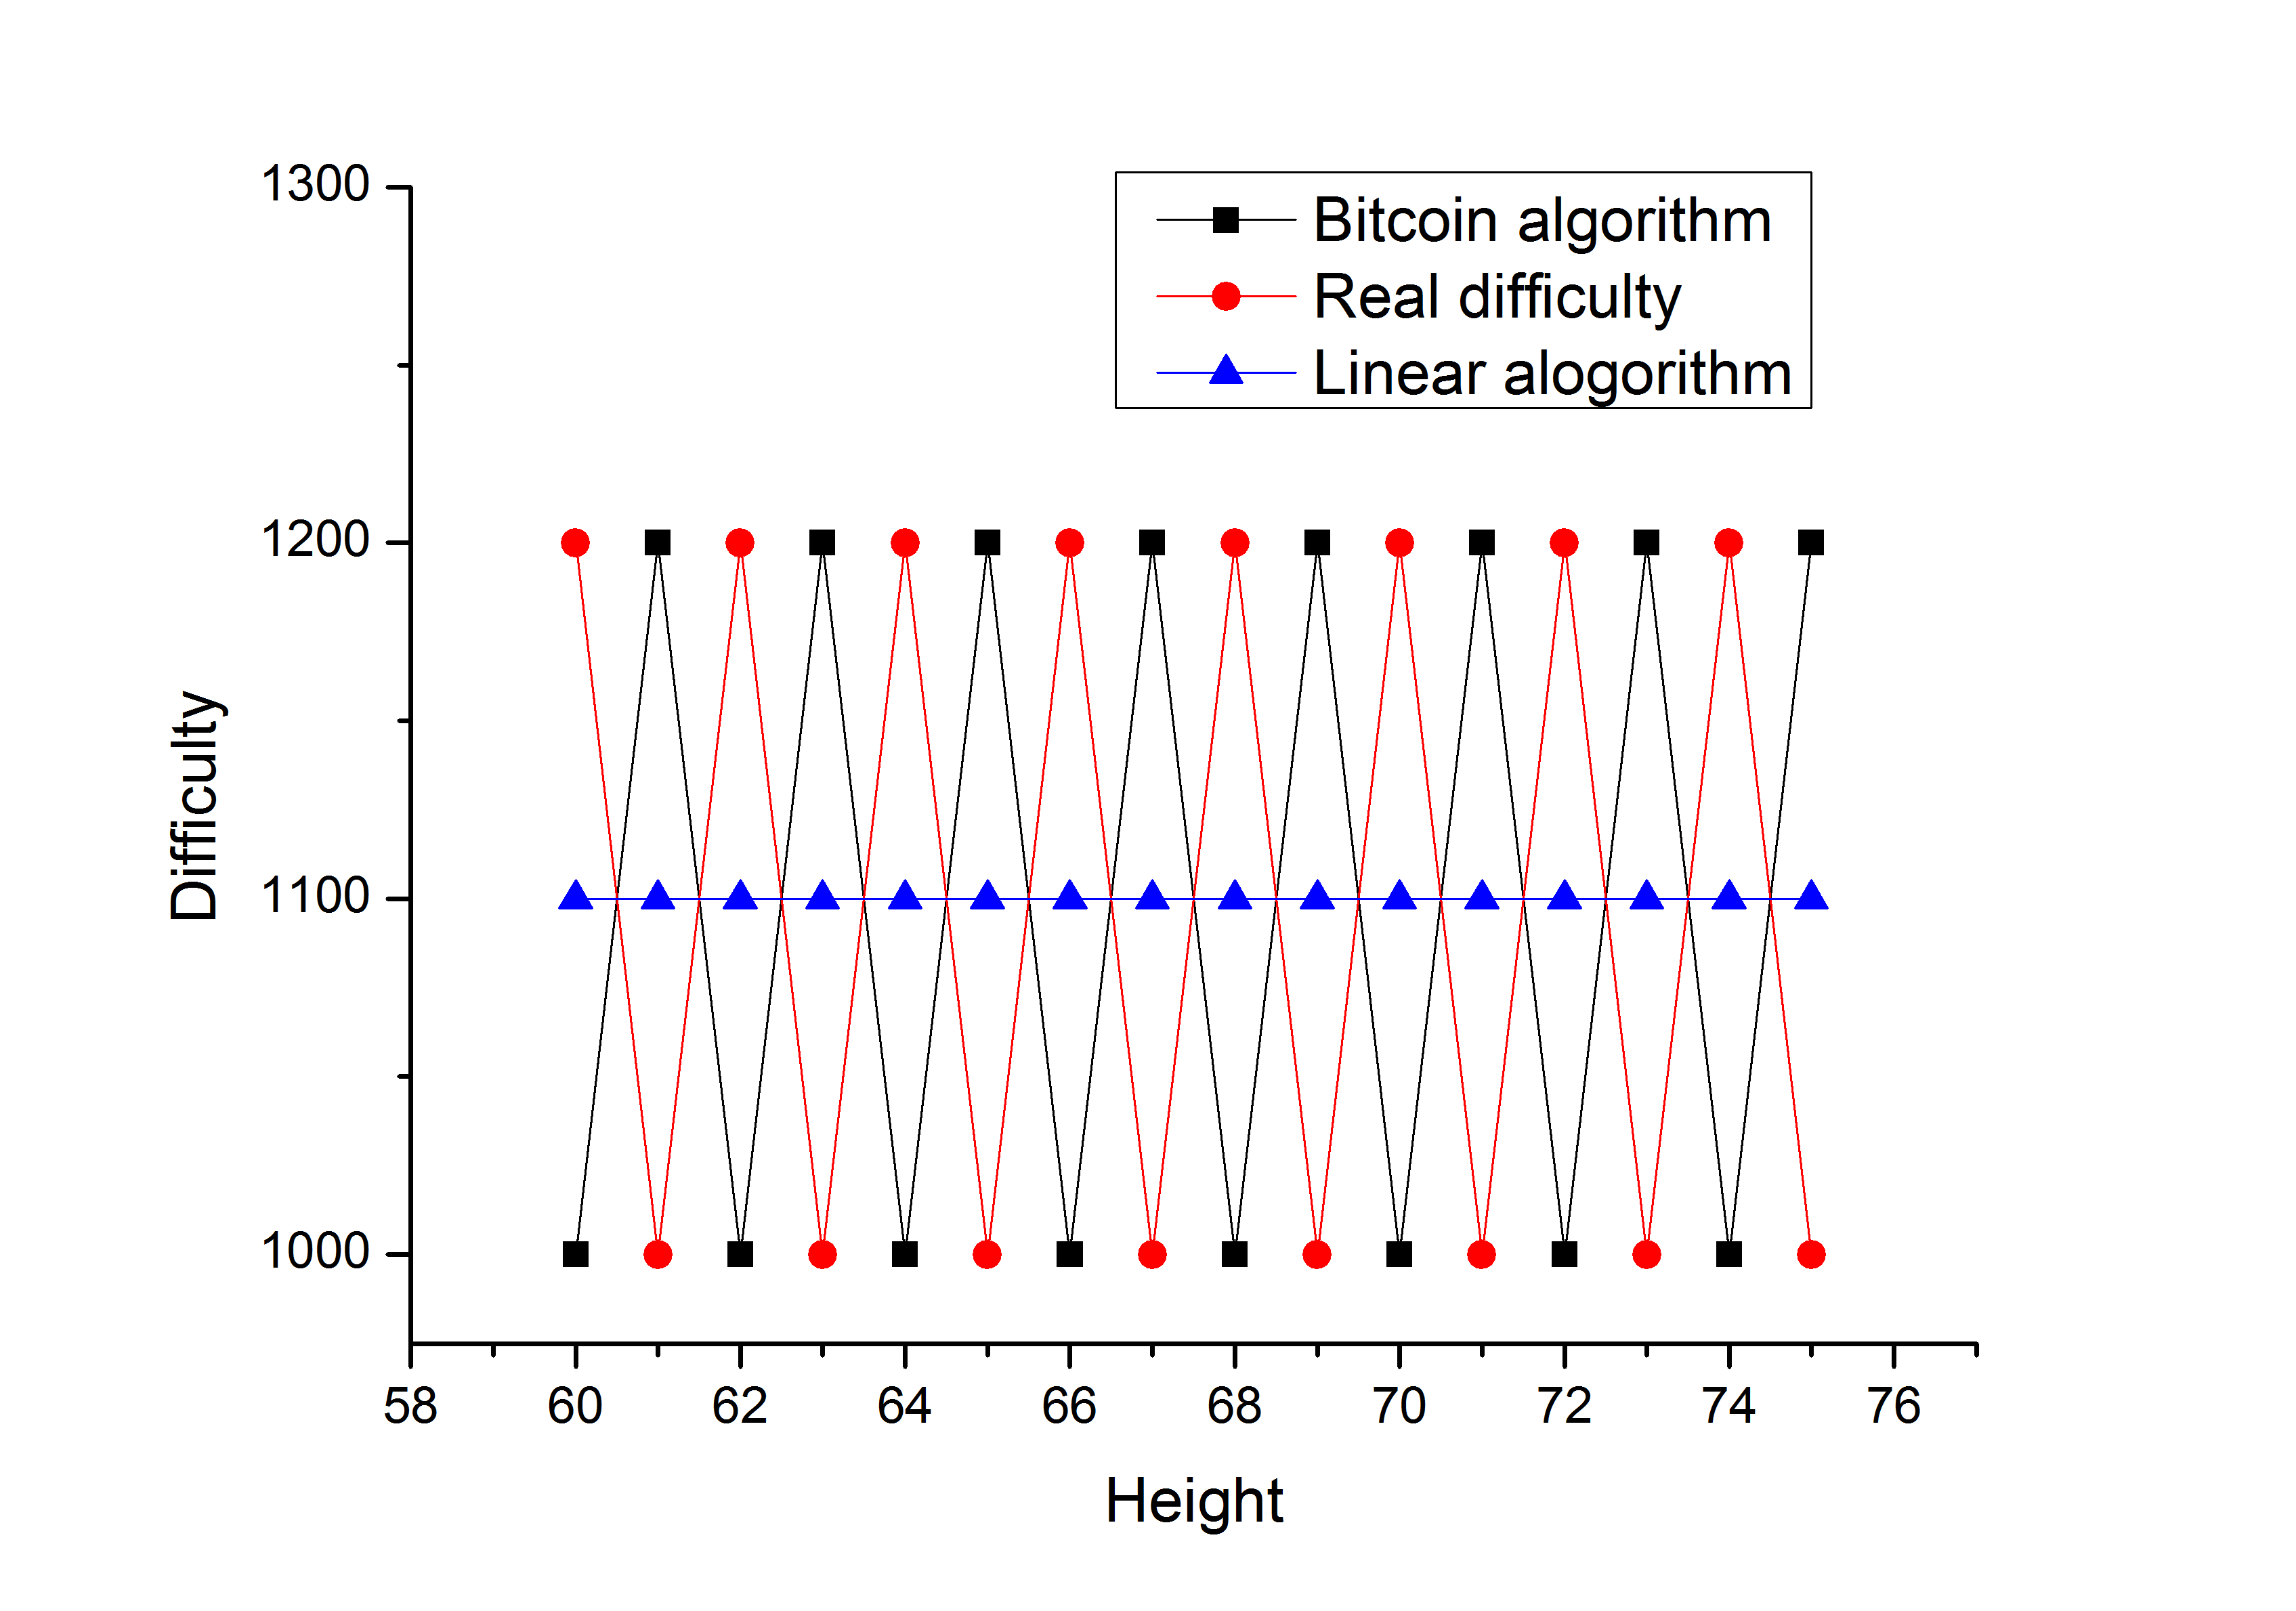
\includegraphics[scale=0.3]{attack.png}}
\caption{Real difficulty (red) and difficulties calculated from bitcoin (black) and linear (blue) algorithms in situation of attack, described in section \ref(sec:attack)}
\label{fig:attack}
\end{figure}

Note that the difficulty calculated with the Bitcoin algorithm is always in antiphase with the real one and the attacker spends his computational power only when difficulty is low.
Bitcoin difficulty update algorithm leads to \textit{10 min 10 sec} mean delay between blocks, which is in good correlation with \ref{eq:ati}.
Linear algorithm also leads to enlarged time interval between blocks \textit{10 min 5 sec}, but it's deviation from desired time is 2 times lower.
Obviously, attacker profit is also 2 times lower in situation with linear difficulty update algorithm, which may be regarded as a good result.

Thus, linear difficulty control algorithm, proposed in Section \ref{sec:improved} is better than the Bitcoin's in all situations both in terms of block rate and in terms of attacker profit.


%\section{Conclusion}
%\label{sec:concl}

%In this paper we analyze a new kind of attacks on the blockchain based on manipulating mining difficulty. This attack decrease computational power spent by an attacker for block mining while increasing mean time interval between blocks. It is especially favorable in situation, when the cost of computational resources invested into mining is around the expected reward and there are enough forks to switch mining between them.

%To improve the stability of block times and decrease the attacker profit, we proposed an alternative difficulty update algorithm, based on linear regression. It was found that this algorithm is better then the Bitcoin one both in terms of block rate and in terms of attacker profit, while it's still simple enough to be computed with integer arithmetic only.

%\section*{Acknowledgments}

\bibliographystyle{elsarticle-num}
\bibliography{sources.bib}


\end{document}